\documentclass[journal]{IEEEtran}
\usepackage{amsmath}
\usepackage{amssymb}
\usepackage{cite}
\usepackage{booktabs}
\usepackage{algorithm}
\usepackage[noend]{algpseudocode}
\usepackage{multicol}
\usepackage{multirow}
\usepackage{array}
\usepackage{mathtools}
\usepackage{dsfont}
\usepackage{color}
\DeclareMathOperator*{\argmax}{arg\,max}
\DeclareMathOperator*{\argmin}{arg\,min}
\renewcommand{\vec}[1]{\boldsymbol{#1}}
\newcommand{\norm}[1]{\left|\left|#1\right|\right|}


\begin{document}
\title{Multi-Output Regression for Spatial Reuse with Federated Learning}

\author{Selim F. Yilmaz, Emre Ozfatura, Kerem Ozfatura, Ozlem Yildiz and Deniz G\"{u}nd\"{u}z}

\markboth{Journal of \LaTeX\ Class Files,~Vol.~14, No.~8, August~2015}%
{Shell \MakeLowercase{\textit{et al.}}: Bare Demo of IEEEtran.cls for IEEE Journals}

\maketitle

\begin{abstract}

\end{abstract}

% Note that keywords are not normally used for peerreview papers.
\begin{IEEEkeywords}
\end{IEEEkeywords}

\IEEEpeerreviewmaketitle



\section{Introduction}
Spatial reuse operation (SR) included in the IEEE 802.11ax-2021 (11ax) amendment \cite{11ax} target to increase the spectral efficiency by allowing parallel transmissions. Hence, SR operation is introduced to address the performance issues in certain scenarios where the basic service sets (BSS), which comprised of an access point (AP) and assigned STAs, are overlapping. In the case of overlapping BSSs (OBSSs),  typical channel access mechanisms based on Carrier Sense Multiple Access (CSMA) underutilizes the spectral resources. To this end, by changing the sensitivity it is possible to reduce the Carrier Sense (CS) area and hence increase the frequency of channel access which, on the other hand, may lead collisions. Hence, the main objective is to design a adaptive mechanism for sensitivity of the CS that maximizes the throughput.




\subsection{Spatial Reuse}
Clear Channel Assessment CS (CCA/CS) protocol aim to ensure that any Wi-Fi device does not transmit while another is already transmitting on the same channel to avoid collusion. Hence, once a Wi-Fi device detect a transmission and decode the preamble of the transmitting device, a busy flag is raised for the channel. The Wi-Fi device can decode the preamble of the corresponding transmission if the signal strength is above certain threshold, which is often referred as the CCA/CS threshold.\\
\indent  SR operation target to adaptively change the sensitivity for channel sensing such that although the sensed power level is above the CCA/CS threshold, the Wi-Fi device may ignore the corresponding transmission and utilize the channel. To this end, we consider a second threshold, namely OBSS/PD threshold, which is utilized to ignore the decoded preamble of the transmission of another device and continue to occupy the channel. We remark that when there are more than one transmission, then capture affect is used that is the strongest signal is considered for CS \cite{wilhelmi2021spatial}. We also want remark that SR-based opportunities are considered when inter-BSS frames are detected, in the case of detecting intra-BSS transmissions, the default
CCA/CS threshold is used.\\
\indent In Fig. \ref{fig:vis}, the visualization of the detection and decoding of the signal is given for IEEE 802.11 devices \cite{wilhelmi2021spatial} when the devices using the same frequency and the power is fixed. AP$_A$ can detect the signals in the gray area but only decode the red area, which is above the CS threshold. Due to the SR operation in 11ax, OBSS threshold prevents the transmission in green area to increase the utilization. 



\subsection{Federated Learning}

The federated learning (FL) framework has been introduced in \cite{FL1} to enable large-scale {\em collaborative learning} in a distributed manner and without sharing local datasets among the clients to address the privacy concerns of the end-users to some extent. Formally, FL aim to solve a problem in the following form
\begin{equation}
\min_{\boldsymbol{\boldsymbol{W}}\in\mathbb{R}^{d}} f(\boldsymbol{W})= \frac{1}{N}\sum^{N}_{i=1}\underbrace{\mathds{E}_{\zeta \sim \mathcal{D}_{i}}F(\boldsymbol{W},\zeta)}_{\mathrel{\mathop:}=f_{i}(\boldsymbol{W})},\label{DSO}
\end{equation}
in a decentralized manner, where $\boldsymbol{w}\in\mathbb{R}^{d}$ denotes the model parameters,  $\zeta$ is a random data sample, $\mathcal{D}_{i}$ denotes the dataset of client $i$, and $F$ is the problem specific empirical loss function. At each iteration of FL,  each client aims to minimize its local loss function $f_{i}(\boldsymbol{w})$ using the {\em stochastic gradient descent} method. Then, the clients seek a consensus on the model under supervision of the central server. The most widely used consensus strategy is averaging the local models periodically which is referred as {\em federated averaging (FedAvg)}. The FedAvg procedure is summarized in Algorithm \ref{alg:fl}.\\
\indent To summarize the FL procedure; at the beginning of round $t$, a subset of the available clients $\mathcal{S}_{t}$ are chosen, default randomly, to participate model update. Then, each chosen client pulls the current global parameter model $\boldsymbol{w}_t$ from the PS and then performs $H$ local updates before the consensus step, as illustrated in Algorithm \ref{alg:fl} (lines 5-6), where 
\begin{equation}
\mathbf{g}^{\tau}_{i,t}=\nabla_{\boldsymbol{W}}f_{n}(\boldsymbol{W}^{\tau-1}_{i,t},\zeta_{i,\tau})
\end{equation}
is the gradient estimate of the $i$-th client at $\tau$-th local iteration based on the randomly sampled local data $\zeta_{i,\tau}$.

\begin{algorithm}[t!]
\caption{Federated Averaging (FedAvg) }\label{alg:fl}
\begin{algorithmic}[1]
\For{$t=1,2,\ldots$}
    \For{$i \in\mathcal{S}_{t}$} in parallel
        \State Pull $\boldsymbol{w}_{t}$ from central server: $\boldsymbol{w}^{0}_{i,t}=\boldsymbol{w}_{t}$
        \For{$\tau=1,\ldots,H$}
            \State Compute SGD: $\mathbf{g}^{\tau}_{i,t}=\nabla_{\boldsymbol{w}}f_{n}(\boldsymbol{w}^{\tau-1}_{i,t},\zeta_{i,\tau})$
            \State Update model: $\boldsymbol{w}^{\tau}_{i,t}=\boldsymbol{w}^{\tau-1}_{i,t}-\eta_{t}\mathbf{g}^{\tau}_{i,t}$
       \EndFor
       \State Push $\boldsymbol{w}^{H}_{i,t}$
    \EndFor
    \State{\textbf{Federated Averaging}:} $\boldsymbol{w}_{t+1}=\frac{1}{ \vert \mathcal{S}_{t} \vert}\sum_{i\in\mathcal{S}_{t}} \boldsymbol{w}^{H}_{i,t}$
\EndFor
\end{algorithmic}
\end{algorithm}

 Then, each participating user pushes its local model parameters to the central server, following $H$ local updates, where those values are aggregated to update the parameter model, i.e.,
\begin{equation}
\boldsymbol{W}_{t+1}=\frac{1}{ \vert \mathcal{S}_{t} \vert}\sum_{i\in\mathcal{S}_{t}} \boldsymbol{W}^{H}_{i,t}.
\end{equation}
\begin{figure*}[h]
\begin{center}
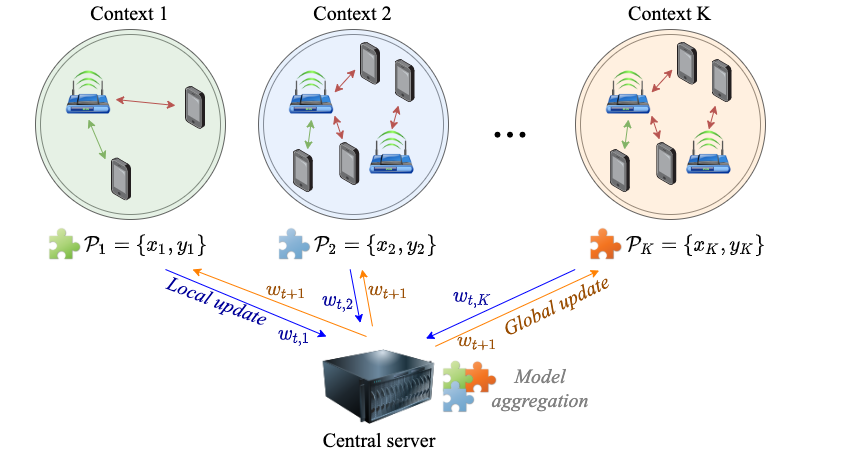
\includegraphics[scale=0.35]{FL_example_ITU.png}
\caption{Illustration of the FL framework for the given SR problem.}
\label{fl_fig}
\end{center}
\end{figure*}


\section{FedIPC Method}
\subsection{Problem Definition}
We denote all vectors by italic bold lowercase characters and all matrices by italic bold uppercase characters.

In the scope of this work, our target is to obtain the optimal OBSS/PD threshold for SR operation that maximize the network throughput. To this end, we aim to design a neural network model which predicts the throughput of each STA in the given BSS for a chosen OBSS/PD threshold from a certain range, thus one can tune the OBSS/PD threshold by using NN architecture.\\
\indent To train the NN model we employ the federated learning framework in the following way; we call a Wi-Fi deployment with specific characteristics such as node locations and number of interfering BSSs as a context. We consider $n$ contexts in total, where for each context, we have $s_i$ STAs per AP for context $i$. We also define $a$ as the maximum number of access point and $b$ as the maximum number of STAs per AP. Note that all contexts may have different number of STAs per AP. We also have interference sensed by APs, RSSI of the STAs assigned to $\mathrm{AP}_\mathrm{A}$, and the average SINR of each STA in $\mathrm{BSS}_A$. We can control control threshold $\tau_i \in \{-82, -81, \ldots, -62\}$. To simplify the problem as in the competition, we can only change the threshold of the $\mathrm{BSS}_A$, and all other BSSs' thresholds are fixed to -82 dBm. Thus, we only consider the STAs in $\mathrm{BSS}_A$.\\
\indent  Regarding the throughput analysis, we first want to remark that a given transmission is successful if the  following two conditions are satisfied; 1) The power sensed at the receiver from the frame being decoded remains above the CCA/CS threshold, 2) Signal-to-Interference-plus-Noise Ratio (SINR)
stays above the capture effect (CE) threshold \cite{wilhelmi2019performance}. Throughput of the successful transmission are determined according to modulation coding scheme (MCS) based on the SINR value and the sensed power, received signal strength indicator (RSSI).  To this end, a look up table, MCS table, is used to map SINR and RSSI values to pair of modulation scheme and encoding rate.\\
\indent Let $t_{j, \tau_{i}}^{(i)} \in \mathbb{R}$ be the throughput of $j^\mathrm{th}$ STA in the $\mathrm{BSS}_A$ of the $i^\mathrm{th}$ context, where threshold of the $\mathrm{BSS}_A$ is chosen as $\tau$. For context i, our objective is to find $\tau_i$ that maximizes the throughput for all STAs in the $\mathrm{BSS}_A$ of context $i$, i.e,
\begin{equation}
    \argmax_{\vec{\tau}} \sum_{i=1}^{n} \sum_{j=1}^{s_i} t_{j, \tau_{i}}^{(i)},
    \label{eq:thresholdeq}
\end{equation}
where $\vec{\tau} = \left[\tau_1, \tau_2, \ldots, \tau_n \right]^T$, $s_i$ is the number of STAs connected to each AP (or the number of STAs in each BSS) in context $i$. Having the knowledge of throughputs $t_{j, \tau^{'}}^{(i)}$, $\forall i,j,\tau_{'}$, which is not likely, one can easily calculate $\vec{\tau}$ using~\eqref{eq:thresholdeq}. Thus, to determine the best threshold for each context $i$, we  estimate $t_{j, \tau^{'}}^{(i)}$ via $\hat{t}_{j, \tau_{i}}^{(i)}$ for all STA $j$ and threshold $\tau^{'}$ combinations.

In the federated learning setting, we model each context as a node, where their data consist of simulations with different thresholds. We assume these nodes cannot communicate with each other, but communicate with a parameter server in rounds, which aggregates the weights of the nodes to create. Then, the parameter server distributes the updated global model to the clients.

\subsection{Neural Network with a Multi-Output Regression Objective}
Here, we describe the neural network model and objective function, which we use in all our clients.

We cannot directly calculate or know the throughput $t_{j, \tau}^{(i)}$. Thus, we estimate it via a model $\hat{t}^{(i)}_{j, \tau} = f^{(i)}_{j,\tau}$, where $i$ is the context index, $j$ is the index of STA connected to $\mathrm{AP}_\mathrm{A}$ and $\tau$ is the threshold. Moreover, estimating one STA's throughput is highly related to estimating another STA's throughput in the same context.  Thus, to exploit this relation, we formulate the throughput regression problem as multi-output regression, as the following:
\begin{equation}
    \vec{f}^{(i)}_\tau (\vec{x}_\tau^{(i)}, \vec{W}_i ) = \left[ f^{(i)}_{1,\tau} \, \, f^{(i)}_{2,\tau} \ldots f^{(i)}_{b,\tau} \right]^T,
\end{equation}
where $i$ is the context index, $\vec{x}_\tau^{(i)}$ is the input vector and $\vec{W}_i$ is the neural network weights of the model at context $i$.

Here, the input vector $\vec{x}_\tau^{(i)} \in \mathbb{R}^{4b+a}$ includes each STA's features in order (for STAs in $\mathrm{BSS}_A$). Each STA's features are as the following: interference sensed by APs, RSSI, the average SINR and the threshold, respectively. When a context has less than $b$ STA per AP. We zero pad for the remaining places until the vector reaches the maximum in the dataset. This is possible since $a$  (the maximum number of APs) and $b$ (the maximum number of STAs per AP) are fixed.

Since every context may have different number of STAs per AP, we mask the nonexistent STAs as the following:
\begin{equation*}
    f^{(i)}_{k, \tau} = \hat{t}^{(i)}_{k, \tau} = t^{(i)}_{k, \tau} = 0 , \, \, \, \, \forall k \in \{s_i + 1, \, \ldots , b \} .
\end{equation*}
This way, we do not backpropagate any loss for nonexistent STAs and become able to train our model for variable number of STAs per AP for every context. 


Then, we define the ground truth vector as:
\begin{equation*}
    \vec{t}^{(i)}_\tau = \left[ t_{1, \tau}^{(i)} \, \, t_{2, \tau}^{(i)} \, \,  \ldots \, \, t_{b, \tau}^{(i)} \right]^T
\end{equation*}

For the context $i$ (local node), our objective is to minimize mean-squared error for regression task for any $(\vec{x}_\tau^{(i)}, \vec{t}^{(i)}_\tau)$ data point among all contexts, i.e.,
\begin{equation*}
\argmin_{\vec{W}_i} \sum_{\forall \tau,i}  \norm{\vec{f}^{(i)}_\tau (\vec{x}_\tau^{(i)}, \vec{W}_i ) - \vec{t}^{(i)}_\tau}_2^2.
\end{equation*}

We use a feed-forward neural network with one hidden layer as our model $\vec{f}^{(i)}_\tau (\vec{x}_\tau^{(i)}, \vec{W}_i)$ with weights $\vec{W}_i = \left[  \vec{W}_i^{(1)} \, \, \vec{W}_i^{(2)} \right]$, where $\vec{f}^{(i)}_\tau (\vec{x}_\tau^{(i)}, \vec{W}_i) = \vec{W}_i^{(2)} \mathrm{ReLU} ( \vec{W}_i^{(1)}\vec{x}_\tau^{(i)}) $, $\vec{W}_i^{(2)} \in \mathbb{R}^{b \times h}$ and  $\vec{W}_i^{(1)} \in \mathbb{R}^{h \times (a+3b)}$. As seen, we use rectified linear unit (ReLU) as our activation function. Note that this neural network can easily be generalized to a neural network with multiple hidden layers, but in our case, the neural network with only 1 hidden layer have worked the best on the validation set.

In the following section, we describe how we combine these local models.

\subsection{FL for Training}
To train our NN architecture for throughput estimation we employ the FL framework particularly FedAvg illustrated in \ref{alg:fl}. To this end,
 we consider each AP of interest in a different context as a participant of the FL framework. Further, for each AP of interest the local dataset consist of the throughput, for each STAs of interest, and all the possible OBSS/PD thresholds\footnote{The size of the local dataset is equal to 21.}. FL framework for the given SR is illustrated in Fig. \ref{fl_fig}.\\
 \indent In general, the participation ratio, the fraction of the users participating model update in each round, and the number of local iterations are two important factors for the performance of the FL. Unless a further communication constraint is introduced we consider full participation for the FL, that is all users participate to model averaging at each communication round.\\
 \indent In the scope of this work, we fixed the batchsize equal to the size of the local dataset, which is 21, and fixed the number of local iteration $H=1$.
 
 \subsection{Implementation Details}
 
We only use the scenario 3 dataset from the ITU-ML5G-PS-004: Federated Learning for Spatial Reuse in a Multi-BSS competition~\footnote{https://challenge.aiforgood.itu.int/match/matchitem/37}. We do not use other scenarios since scenario 3 is the most complex data. The target variable is the throughput as defined in problem definition. It contains variable number of STAs per AP and different node locations. All different node locations are combined with all possible thresholds. It has between 2 and 6 APs, between 1 and 4 STAs per AP, i.e., $a \in \{2,3,4,5,6\}$ and $s_i \in \{1,2,3,4\} \, \forall \, i$. Moreover, in scenario 3 dataset, different STA/AP location configurations (up to 20 different) have been generated and data points are generated for all thresholds using these STA/AP location configurations. Note that different number of .

We split the dataset into training (80\% of the contexts), first validation (10\% of the contexts) and second validation (10\% of the contexts) sets, for which we explain the reasoning in the following section.

We evaluate the prediction results of our method via the main absolute error (MAE) metric. Recall that we estimate the throughputs by multi-output regression task and each context may have different number of throughputs to be predicted. Thus, we flatten the predictions for existing STAs before calculating the MAE. We normalize the data by minmax normalization. We use to implement the standard SGD implementation of Pytorch~\cite{paszke2017automatic} to implement federated averaging.

We have two different validation sets, where each validation set contains the data of 100 contexts. We use the first validation set for early stopping of the global model. We evaluate our global model after every 20 rounds and stop training if no improvement in validation MAE is achieved after 100 rounds. Then, we simply choose the final global model that has the lowest validation MAE throughout the training. 

We use the second validation set to perform hyperparameter tuning. We tune our method by using Tree Parzen Estimator of the Optuna library~\cite{akiba2019optuna} and choose the model with the lowest MAE on the second validation set. Finally, we compute the throughput estimations on the test set of the competition.

\bibliography{ref.bib}
\balance
\bibliographystyle{IEEEtran}

\end{document}


